\documentclass[border=6pt]{standalone}
\usepackage{amsmath,amssymb}
\usepackage{xcolor}
\usepackage{tikz}
\usetikzlibrary{arrows.meta,backgrounds,decorations.pathreplacing}
\definecolor{cblue}{HTML}{1976D2}
\definecolor{cred}{HTML}{E53935}
\definecolor{cpurple}{HTML}{5E35B1}
\definecolor{cgrey}{HTML}{757575}
\tikzset{every picture/.append style={show background rectangle,
    background rectangle/.style={fill=white}, inner frame sep=4pt}}
% The search as a stream: the recurrence diagram of one window on the grid of the samples, the start across
% and the lag up, 16 starts by 7 lags, drawn with h = 9, W_t = 4 and W_T = 1. The cells are shaded by a made-up
% distance, blue below the threshold. The candidate at the centre of the red box is the one that the new column
% decides: the box spans W_t starts each way and W_T lags each way, a repeat inside it is dropped, and a
% candidate of another period, outside it, is kept. Under the diagram, the samples of the stream: the buffer
% holds them from the start of the candidate being decided to the new sample k, which is the last end of the
% start k - h and completes its column.
\begin{document}
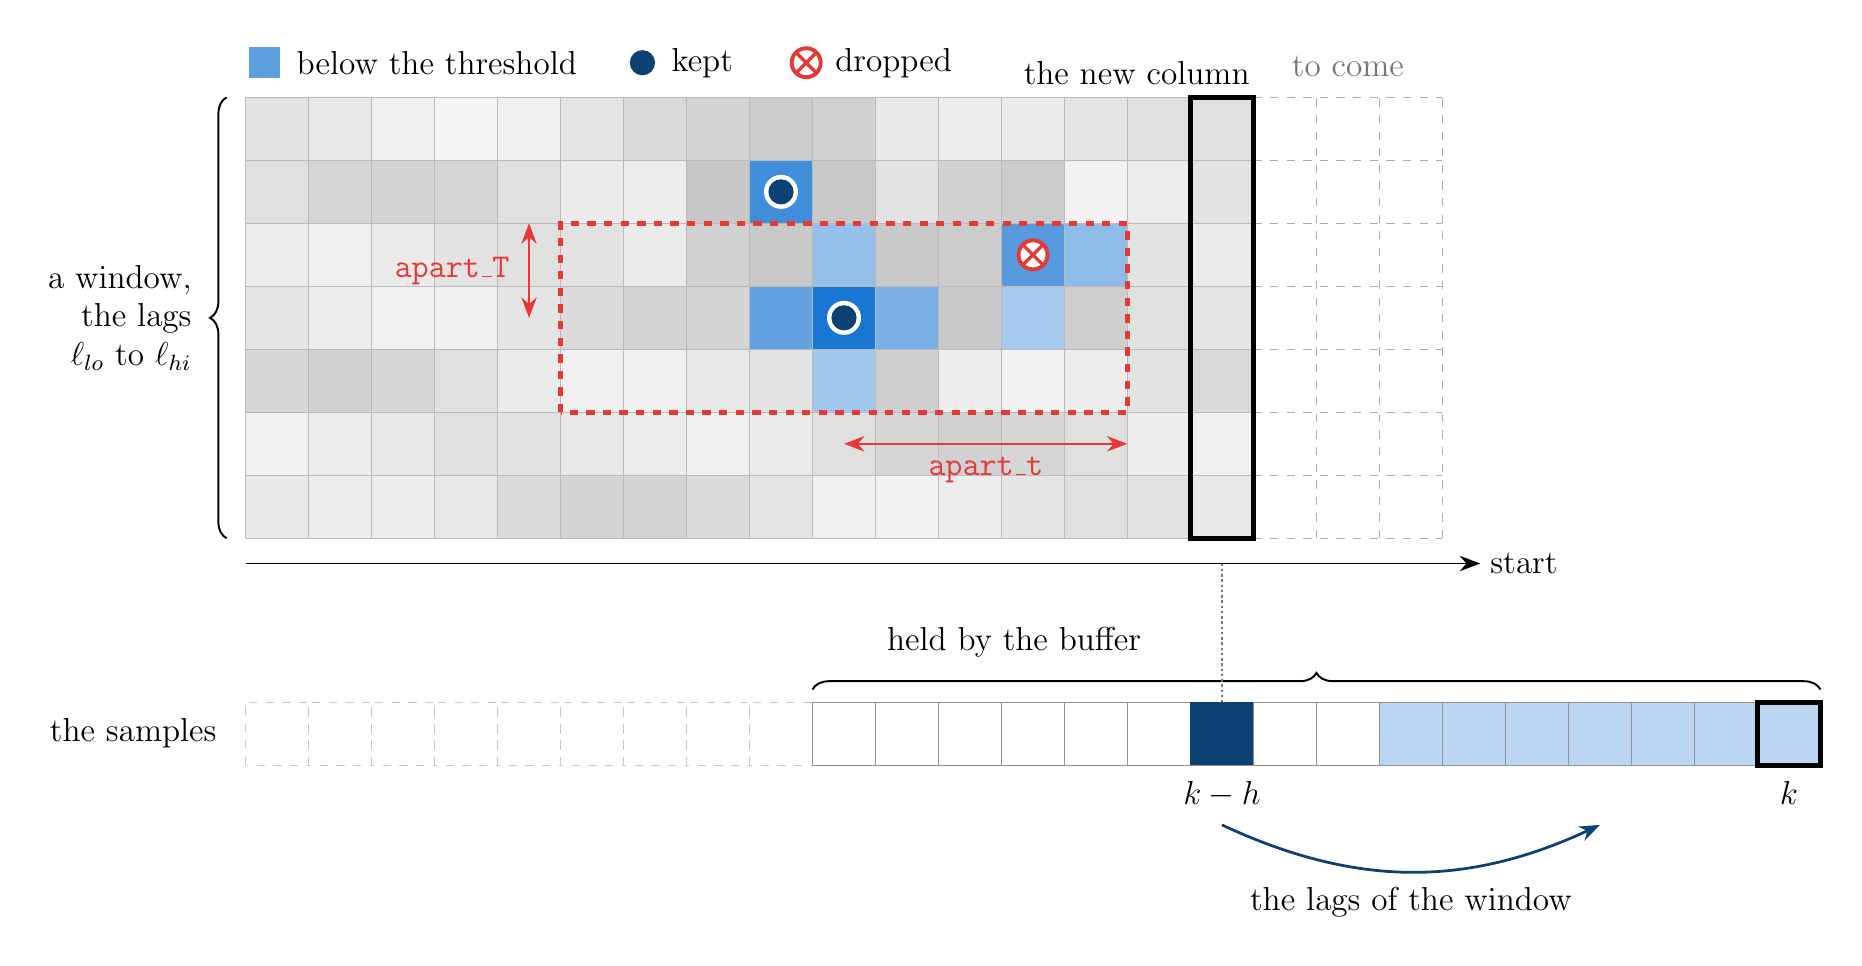
\begin{tikzpicture}[>={Stealth[length=2.6mm]}, every node/.style={font=\large}, x=0.8cm, y=0.8cm,
                    line width=0.7pt]
  % ---- the cells of the window: blue below the threshold, the darker the closer ----
  \fill[black!9] (0, 0) rectangle ++(1, 1);
  \fill[black!5] (0, 1) rectangle ++(1, 1);
  \fill[black!16] (0, 2) rectangle ++(1, 1);
  \fill[black!10] (0, 3) rectangle ++(1, 1);
  \fill[black!7] (0, 4) rectangle ++(1, 1);
  \fill[black!12] (0, 5) rectangle ++(1, 1);
  \fill[black!11] (0, 6) rectangle ++(1, 1);
  \fill[black!7] (1, 0) rectangle ++(1, 1);
  \fill[black!7] (1, 1) rectangle ++(1, 1);
  \fill[black!18] (1, 2) rectangle ++(1, 1);
  \fill[black!7] (1, 3) rectangle ++(1, 1);
  \fill[black!6] (1, 4) rectangle ++(1, 1);
  \fill[black!16] (1, 5) rectangle ++(1, 1);
  \fill[black!9] (1, 6) rectangle ++(1, 1);
  \fill[black!7] (2, 0) rectangle ++(1, 1);
  \fill[black!9] (2, 1) rectangle ++(1, 1);
  \fill[black!16] (2, 2) rectangle ++(1, 1);
  \fill[black!5] (2, 3) rectangle ++(1, 1);
  \fill[black!8] (2, 4) rectangle ++(1, 1);
  \fill[black!17] (2, 5) rectangle ++(1, 1);
  \fill[black!6] (2, 6) rectangle ++(1, 1);
  \fill[black!9] (3, 0) rectangle ++(1, 1);
  \fill[black!12] (3, 1) rectangle ++(1, 1);
  \fill[black!12] (3, 2) rectangle ++(1, 1);
  \fill[black!6] (3, 3) rectangle ++(1, 1);
  \fill[black!11] (3, 4) rectangle ++(1, 1);
  \fill[black!16] (3, 5) rectangle ++(1, 1);
  \fill[black!4] (3, 6) rectangle ++(1, 1);
  \fill[black!14] (4, 0) rectangle ++(1, 1);
  \fill[black!11] (4, 1) rectangle ++(1, 1);
  \fill[black!8] (4, 2) rectangle ++(1, 1);
  \fill[black!10] (4, 3) rectangle ++(1, 1);
  \fill[black!12] (4, 4) rectangle ++(1, 1);
  \fill[black!12] (4, 5) rectangle ++(1, 1);
  \fill[black!6] (4, 6) rectangle ++(1, 1);
  \fill[black!17] (5, 0) rectangle ++(1, 1);
  \fill[black!9] (5, 1) rectangle ++(1, 1);
  \fill[black!6] (5, 2) rectangle ++(1, 1);
  \fill[black!14] (5, 3) rectangle ++(1, 1);
  \fill[black!11] (5, 4) rectangle ++(1, 1);
  \fill[black!8] (5, 5) rectangle ++(1, 1);
  \fill[black!10] (5, 6) rectangle ++(1, 1);
  \fill[black!17] (6, 0) rectangle ++(1, 1);
  \fill[black!7] (6, 1) rectangle ++(1, 1);
  \fill[black!6] (6, 2) rectangle ++(1, 1);
  \fill[black!17] (6, 3) rectangle ++(1, 1);
  \fill[black!8] (6, 4) rectangle ++(1, 1);
  \fill[black!7] (6, 5) rectangle ++(1, 1);
  \fill[black!15] (6, 6) rectangle ++(1, 1);
  \fill[black!14] (7, 0) rectangle ++(1, 1);
  \fill[black!6] (7, 1) rectangle ++(1, 1);
  \fill[black!9] (7, 2) rectangle ++(1, 1);
  \fill[black!17] (7, 3) rectangle ++(1, 1);
  \fill[black!18] (7, 4) rectangle ++(1, 1);
  \fill[black!22] (7, 5) rectangle ++(1, 1);
  \fill[black!17] (7, 6) rectangle ++(1, 1);
  \fill[black!10] (8, 0) rectangle ++(1, 1);
  \fill[black!8] (8, 1) rectangle ++(1, 1);
  \fill[black!11] (8, 2) rectangle ++(1, 1);
  \fill[cblue!68] (8, 3) rectangle ++(1, 1);
  \fill[black!21] (8, 4) rectangle ++(1, 1);
  \fill[cblue!83] (8, 5) rectangle ++(1, 1);
  \fill[black!20] (8, 6) rectangle ++(1, 1);
  \fill[black!6] (9, 0) rectangle ++(1, 1);
  \fill[black!12] (9, 1) rectangle ++(1, 1);
  \fill[cblue!41] (9, 2) rectangle ++(1, 1);
  \fill[cblue!100] (9, 3) rectangle ++(1, 1);
  \fill[cblue!46] (9, 4) rectangle ++(1, 1);
  \fill[black!21] (9, 5) rectangle ++(1, 1);
  \fill[black!18] (9, 6) rectangle ++(1, 1);
  \fill[black!5] (10, 0) rectangle ++(1, 1);
  \fill[black!16] (10, 1) rectangle ++(1, 1);
  \fill[black!19] (10, 2) rectangle ++(1, 1);
  \fill[cblue!58] (10, 3) rectangle ++(1, 1);
  \fill[black!21] (10, 4) rectangle ++(1, 1);
  \fill[black!11] (10, 5) rectangle ++(1, 1);
  \fill[black!9] (10, 6) rectangle ++(1, 1);
  \fill[black!7] (11, 0) rectangle ++(1, 1);
  \fill[black!18] (11, 1) rectangle ++(1, 1);
  \fill[black!7] (11, 2) rectangle ++(1, 1);
  \fill[black!21] (11, 3) rectangle ++(1, 1);
  \fill[black!20] (11, 4) rectangle ++(1, 1);
  \fill[black!18] (11, 5) rectangle ++(1, 1);
  \fill[black!7] (11, 6) rectangle ++(1, 1);
  \fill[black!10] (12, 0) rectangle ++(1, 1);
  \fill[black!16] (12, 1) rectangle ++(1, 1);
  \fill[black!5] (12, 2) rectangle ++(1, 1);
  \fill[cblue!39] (12, 3) rectangle ++(1, 1);
  \fill[cblue!73] (12, 4) rectangle ++(1, 1);
  \fill[black!20] (12, 5) rectangle ++(1, 1);
  \fill[black!8] (12, 6) rectangle ++(1, 1);
  \fill[black!12] (13, 0) rectangle ++(1, 1);
  \fill[black!12] (13, 1) rectangle ++(1, 1);
  \fill[black!7] (13, 2) rectangle ++(1, 1);
  \fill[black!19] (13, 3) rectangle ++(1, 1);
  \fill[cblue!49] (13, 4) rectangle ++(1, 1);
  \fill[black!5] (13, 5) rectangle ++(1, 1);
  \fill[black!10] (13, 6) rectangle ++(1, 1);
  \fill[black!11] (14, 0) rectangle ++(1, 1);
  \fill[black!7] (14, 1) rectangle ++(1, 1);
  \fill[black!11] (14, 2) rectangle ++(1, 1);
  \fill[black!12] (14, 3) rectangle ++(1, 1);
  \fill[black!11] (14, 4) rectangle ++(1, 1);
  \fill[black!7] (14, 5) rectangle ++(1, 1);
  \fill[black!12] (14, 6) rectangle ++(1, 1);
  \fill[black!9] (15, 0) rectangle ++(1, 1);
  \fill[black!6] (15, 1) rectangle ++(1, 1);
  \fill[black!15] (15, 2) rectangle ++(1, 1);
  \fill[black!10] (15, 3) rectangle ++(1, 1);
  \fill[black!8] (15, 4) rectangle ++(1, 1);
  \fill[black!11] (15, 5) rectangle ++(1, 1);
  \fill[black!12] (15, 6) rectangle ++(1, 1);
  \draw[cgrey!50, line width=0.3pt, step=1] (0, 0) grid (16, 7);
  % ---- the columns to come ----
  \draw[cgrey!60, dashed, line width=0.4pt, step=1] (16, 0) grid (19, 7);
  \node[cgrey] at (17.5, 7.5) {to come};
  % ---- the column that the new sample completes ----
  \draw[black, line width=1.8pt] (15, 0) rectangle ++(1, 7);
  \node[anchor=south east] at (16.1, 7.05) {the new column};
  % ---- the box of the closest candidate, apart_t each way along the start and apart_T along the lag ----
  \draw[cred, dashed, line width=1.6pt] (5, 2) rectangle (14, 5);
  \fill[white] (9.5, 3.5) circle (0.27); \fill[cblue!55!black] (9.5, 3.5) circle (0.2);
  \fill[white] (8.5, 5.5) circle (0.27); \fill[cblue!55!black] (8.5, 5.5) circle (0.2);
  \draw[cred, line width=1.4pt, fill=white] (12.5, 4.5) circle (0.23);
  \draw[cred, line width=1.2pt] (12.35, 4.35) -- (12.65, 4.65) (12.35, 4.65) -- (12.65, 4.35);
  % ---- the two widths ----
  \draw[cred, <->] (9.5, 1.5) -- (14, 1.5) node[midway, below=1pt] {\texttt{apart\_t}};
  \draw[cred, <->] (4.5, 3.5) -- (4.5, 5);
  \node[cred, anchor=east] at (4.35, 4.25) {\texttt{apart\_T}};
  % ---- the window and the axes ----
  \draw[decorate, decoration={brace, amplitude=6pt}] (-0.3, 0) -- (-0.3, 7) node[midway, left=9pt, align=right] {a window,\\ the lags\\ $\ell_{lo}$ to $\ell_{hi}$};
  \draw[->] (0, -0.4) -- (19.6, -0.4) node[right] {start};
  \fill[cblue!70] (0.05, 7.3) rectangle ++(0.5, 0.5); \node[anchor=west] at (0.65, 7.55) {below the threshold};
  \fill[cblue!55!black] (6.3, 7.55) circle (0.2); \node[anchor=west] at (6.6, 7.55) {kept};
  \draw[cred, line width=1.4pt, fill=white] (8.9, 7.55) circle (0.23); \draw[cred, line width=1.2pt] (8.75, 7.4) -- (9.05, 7.7) (8.75, 7.7) -- (9.05, 7.4);
  \node[anchor=west] at (9.2, 7.55) {dropped};
  % ---- the samples: the column of a start is made of its sample and of the samples a lag later ----
  \draw[cgrey!40, dashed, line width=0.4pt] (0, -3.6) rectangle ++(1, 1);
  \draw[cgrey!40, dashed, line width=0.4pt] (1, -3.6) rectangle ++(1, 1);
  \draw[cgrey!40, dashed, line width=0.4pt] (2, -3.6) rectangle ++(1, 1);
  \draw[cgrey!40, dashed, line width=0.4pt] (3, -3.6) rectangle ++(1, 1);
  \draw[cgrey!40, dashed, line width=0.4pt] (4, -3.6) rectangle ++(1, 1);
  \draw[cgrey!40, dashed, line width=0.4pt] (5, -3.6) rectangle ++(1, 1);
  \draw[cgrey!40, dashed, line width=0.4pt] (6, -3.6) rectangle ++(1, 1);
  \draw[cgrey!40, dashed, line width=0.4pt] (7, -3.6) rectangle ++(1, 1);
  \draw[cgrey!40, dashed, line width=0.4pt] (8, -3.6) rectangle ++(1, 1);
  \draw[cgrey!80, line width=0.4pt] (9, -3.6) rectangle ++(1, 1);
  \draw[cgrey!80, line width=0.4pt] (10, -3.6) rectangle ++(1, 1);
  \draw[cgrey!80, line width=0.4pt] (11, -3.6) rectangle ++(1, 1);
  \draw[cgrey!80, line width=0.4pt] (12, -3.6) rectangle ++(1, 1);
  \draw[cgrey!80, line width=0.4pt] (13, -3.6) rectangle ++(1, 1);
  \draw[cgrey!80, line width=0.4pt] (14, -3.6) rectangle ++(1, 1);
  \draw[cgrey!80, line width=0.4pt] (15, -3.6) rectangle ++(1, 1);
  \draw[cgrey!80, line width=0.4pt] (16, -3.6) rectangle ++(1, 1);
  \draw[cgrey!80, line width=0.4pt] (17, -3.6) rectangle ++(1, 1);
  \draw[cgrey!80, line width=0.4pt] (18, -3.6) rectangle ++(1, 1);
  \draw[cgrey!80, line width=0.4pt] (19, -3.6) rectangle ++(1, 1);
  \draw[cgrey!80, line width=0.4pt] (20, -3.6) rectangle ++(1, 1);
  \draw[cgrey!80, line width=0.4pt] (21, -3.6) rectangle ++(1, 1);
  \draw[cgrey!80, line width=0.4pt] (22, -3.6) rectangle ++(1, 1);
  \draw[cgrey!80, line width=0.4pt] (23, -3.6) rectangle ++(1, 1);
  \draw[cgrey!80, line width=0.4pt] (24, -3.6) rectangle ++(1, 1);
  \fill[cblue!55!black] (15, -3.6) rectangle ++(1, 1);
  \fill[cblue!30] (18, -3.6) rectangle ++(1, 1); \draw[cgrey!80, line width=0.4pt] (18, -3.6) rectangle ++(1, 1);
  \fill[cblue!30] (19, -3.6) rectangle ++(1, 1); \draw[cgrey!80, line width=0.4pt] (19, -3.6) rectangle ++(1, 1);
  \fill[cblue!30] (20, -3.6) rectangle ++(1, 1); \draw[cgrey!80, line width=0.4pt] (20, -3.6) rectangle ++(1, 1);
  \fill[cblue!30] (21, -3.6) rectangle ++(1, 1); \draw[cgrey!80, line width=0.4pt] (21, -3.6) rectangle ++(1, 1);
  \fill[cblue!30] (22, -3.6) rectangle ++(1, 1); \draw[cgrey!80, line width=0.4pt] (22, -3.6) rectangle ++(1, 1);
  \fill[cblue!30] (23, -3.6) rectangle ++(1, 1); \draw[cgrey!80, line width=0.4pt] (23, -3.6) rectangle ++(1, 1);
  \fill[cblue!30] (24, -3.6) rectangle ++(1, 1); \draw[cgrey!80, line width=0.4pt] (24, -3.6) rectangle ++(1, 1);
  \draw[black, line width=1.8pt] (24, -3.6) rectangle ++(1, 1);
  \node[anchor=north] at (15.5, -3.7) {$k - h$};
  \node[anchor=north] at (24.5, -3.7) {$k$};
  \node[anchor=east, align=right] at (-0.3, -3.1) {the samples};
  \draw[decorate, decoration={brace, amplitude=6pt}] (9, -2.4000000000000004) -- (25, -2.4000000000000004) node[pos=0.2, above=8pt] {held by the buffer};
  \draw[cblue!55!black, ->, line width=1pt] (15.5, -4.55) to[bend right=25] node[midway, below=2pt, black] {the lags of the window} (21.5, -4.55);
  \draw[cgrey, densely dotted, line width=0.9pt] (15.5, -0.4) -- (15.5, -2.6);
\end{tikzpicture}
\end{document}
